\documentclass[../main.tex]{subfiles}

\begin{document}

\section{Metadata}
\label{section:lauxus:metadata}

\par As seen in the previous sections, we need a data structure in order to store information corresponding to each filesystem node (e.g: file entitlement, file encryption keys and users registration). We will call this structure a metadata and will be covered in detail in this section. This structure will be secured thanks to the root key. As a quick reminder, it is the key that will be shared with other authorised users in order to access the filesystem.


\subsection{Structure}
\label{section:lauxus:metadata_structure}

\par As metadata are holding sensitive information about each node, it must be encrypted. However, some information are not required to be encrypted. This is why we designed a metadata to be composed of three parts:
\begin{itemize}
    \item A \textbf{preamble section} holding non sensitive information such as: the size of the associated file for Filenode, the UUIDs of its children for a Dirnode, etc. This section will be only be secured with integrity protection. In this way, we are sure that this section can't be tampered with without being detected.
    \item A \textbf{secured section} holding the sensitive information that can't be divulged. It will thus be encrypted.
    \item A \textbf{cryptographic context} containing the information to securely store the other two sections. Such as the encryption key and the authentication tag to authenticate the preamble section. On top of that, this section will be authenticated and encrypted with the root key. In this way, this section will be at the same time tamper-evident and secured.
\end{itemize}
\par The idea is to have the metadata content secured by its cryptographic context, which in turn, will be secured thanks to the filesystem root key. The root key being protected by the Enclave itself. We applied this procedure to reduce the usage of the root key, and thereby increase its security as it is a long lived key. The root key is set at the filesystem creation time and is never changed afterwards. Indeed, using a same key to encrypt a lot of plaintext leaks, after some time, a lot of information about the key itself to the attacker.


\subsection{Application to the nodes}
\label{section:lauxus:nodes_hierarchy}

\begin{figure}[h]
    \centering
    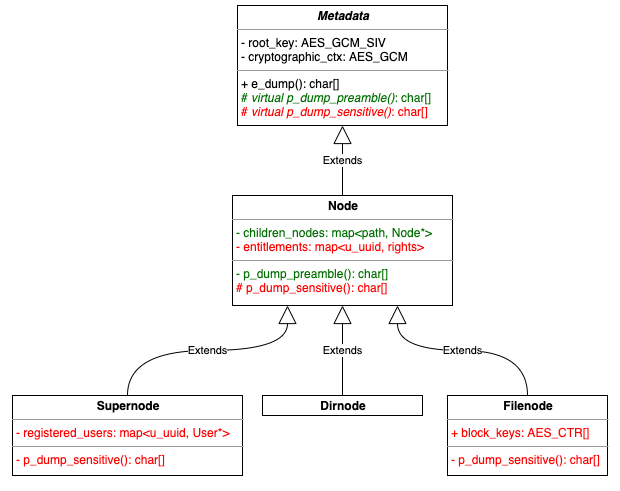
\includegraphics[width=.75\textwidth]{images/lauxus/metadata_hierarchy}
    
    \caption{Metadata UML hierarchy}
    \label{figure:lauxus:metadata_hierarchy}
\end{figure}
\par Now that we have seen the structure of a metadata, we can explain in details which data of a node is located in which section, as described in the Figure \ref{figure:lauxus:metadata_hierarchy}.
\par First of all, we see that the metadata is an abstract class used as a wrapper to secure the preamble and secured sections provided by children classes. In this way, the children just need to return the plaintext content of their desired section and everything will be secured using the metadata wrapper.
\par Second, nodes are extending this abstract class through a generic Node class which contains information common to each node type: a list of child nodes and an entitlement list. The first list will be stored in the preamble section and the latter one in the sensitive section. We put the children nodes inside the preamble section because we don't care if an attacker can discover the hierarchy of the filesystem, as long at the directories and files names are obfuscated.
\par Last, each node type may store complementary information inside the sensitive section. According to the UML diagram in Figure \ref{figure:lauxus:metadata_hierarchy}, we see that the supernode stores the list of registered users and the filenode will store the list of block keys of its associated file.


\subsection{Encryption procedure}
\label{section:lauxus:metadata_encryption}

\par As we have seen in the structure of a metadata, the cryptographic context is used to encrypt the required information. Here, we will more focus on the exact procedure and justify the encryption scheme we used.
\par First of all, we start by securing the secured section using an authenticated scheme. The authenticated additional material will be the preamble section. This allows us to protect at the same time both sections: encrypt the secured section and produce a Message Authentication Code (MAC) linked with the preamble section, making the both ones tamper-evident. Afterwards, this MAC will be stored inside the cryptographic context. The authenticated scheme used is AES GCM which is widely used in today's current cryptographic system. As it is constructed on top of AES CTR, its main weakness is its nonce non re-usability. Indeed, we can't encrypt multiple times using the same IV/Key pair even if the adversary doesn't know the IV, see Appendix \ref{appendix:ctr_nonce_weakness} for demonstration. This justifies the update of the IV of the cryptographic context on every metadata content update.
\par Now that the metadata information are secured, we must secure the information used to secure the metadata content. As discussed above, we will encrypt them using the root key. For portability reason, the root key is in fact composed of an encryption key and an IV. This allows us to use a single IV for all the metadata in the filesystem. This means that we can no longer use the AES GCM encryption algorithm as we are reusing the same IV. We will rely on a variant of AES GCM: AES GCM SIV (similar to AES GCM but with IV reusability). With this algorithm, we will encrypt the cryptographic context and save the generated MAC inside the metadata structure. To synthesise this all process, the Figure \ref{figure:lauxus:metadate_encryption} represents the full structure of a metadata (as saved on the remote storage).
\begin{figure}[ht]
    \centering
    \begin{minipage}{.5\textwidth}
        \centering
        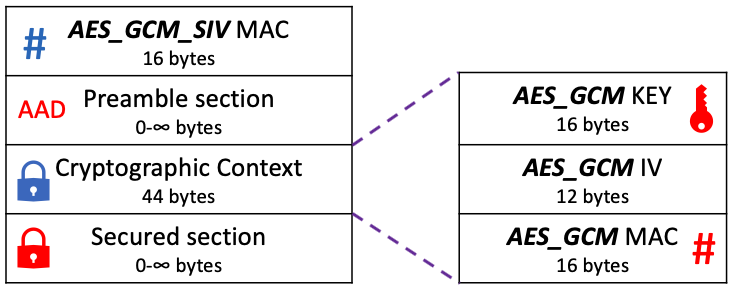
\includegraphics[width=.9\linewidth]{images/lauxus/metadata_encryption}
        \captionof{figure}{Metadata structure}
        \label{figure:lauxus:metadate_encryption}
    \end{minipage}%
    \begin{minipage}{.5\textwidth}
        \centering
        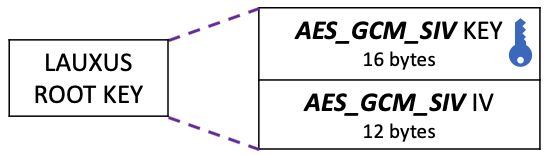
\includegraphics[width=.9\linewidth]{images/lauxus/root_key}
        \captionof{figure}{Root Key representation}
        \label{figure:lauxus:root_key}
    \end{minipage}
\end{figure}

\end{document} 